\documentclass[11pt]{beamer}  %% versione proiettore
%%\documentclass[11pt,handout]{beamer} %% versione stampa
\usepackage{lucidiJb-2ed}
\usepackage[normalem]{ulem}

\usepackage{relsize}

\mode<article>
{
  \usepackage{fullpage}
  \usepackage{hyperref}
}

\mode<presentation>
{
  \setbeamertemplate{background canvas}[vertical shading][bottom=red!10,top=blue!10]
  \usetheme{Ethereum}
  \usefonttheme[onlysmall]{structurebold}
}

\subtitle{Learning Ethereum}
\title{Smart Contract Security}
\institute{Universit\`a di Verona, Italy}
\date{January 2020}

\setbeamercovered{invisible}

\def\codesize{\smaller}
\def\<#1>{\codeid{#1}}
\newcommand{\codeid}[1]{\ifmmode{\mbox{\codesize\ttfamily{#1}}}\else{\codesize\ttfamily #1}\fi}

\begin{document}

\begin{frame}
  \titlepage
\end{frame}

\begin{frame}\frametitle{Security best practice}

  \begin{itemize}
  \item Minimalism: the simpler, the better
  \item Code reuse: DRY, use well-known libraries
  \item Study: be aware of well-known issues and solutions
  \item Readability: simpler audit
  \item Test: try corner cases
  \item Analysis: static or dynamic, still in infancy
  \end{itemize}

  \bigskip

  \begin{redbox}{}
    Considering the importance of security for smart contracts,
    it is questionable to have invented Solidity (hard, new, with convoluted
    semantics) for writing such delicate pieces of software.
  \end{redbox}

  \bigskip

  \begin{center}
    Remember the DAO.
  \end{center}
  
\end{frame}

\begin{frame}\frametitle{Issue \#1: Reentrancy}

  \begin{redbox}{}
    Our contract calls an unknown contract. The latter, unexpectedly, calls
    back into our contract again. Particularly dangerous if this cycle
    passes through a call sending ETH, that would be repeated as many
    times as the unknown contract decides.
  \end{redbox}

  \bigskip

  \begin{greenbox}{Three ways of sending ETH}
    \begin{description}
    \item[\<c.send(amount)>] forwards $2300$ units of gas,
      \alert{currently not enough for reentrancy}; possibly
      deprecated in the future
    \item[\<c.transfer(amount)>] forwards $2300$ units of gas,
      \alert{currently not enough for reentrancy}; possibly
      deprecated in the future
    \item[\<c.call.value(amount)()>] forwards all remaining units of gas,
      typically \alert{enough for reentrancy}; programmers like it since
      it allows one to activate the complex fallback function of any
      contract, not just the default fallback function
    \end{description}
  \end{greenbox}
  
\end{frame}

\begin{frame}\frametitle{Reentrancy: prevention}

  \begin{greenbox}{Use the checks/effects/interactions pattern}
    \begin{center}
      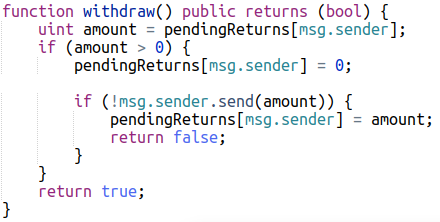
\includegraphics[scale=0.4,clip=false]{pictures/simple-auction-withdraw-only.png}
    \end{center}
  \end{greenbox}

  \medskip

  \begin{greenbox}{Use a mutex to ban reentrancy}
    \begin{center}
      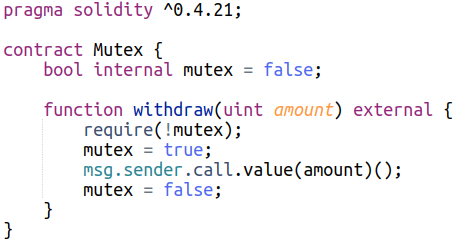
\includegraphics[scale=0.35,clip=false]{pictures/mutex.png}
    \end{center}
  \end{greenbox}
  
\end{frame}

\begin{frame}\frametitle{Issue \#2: Arithmetic over/underflows}

  \begin{redbox}{}
    An operation tries to compute a fixed-size value that is outside the
    bounds for its type.
  \end{redbox}

  \bigskip

  \begin{greenbox}{What if an account with $0$ balance tries to send $1$ ETH to another account?}
    \begin{center}
      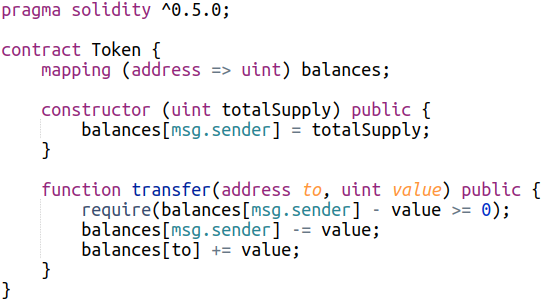
\includegraphics[scale=0.5,clip=false]{pictures/under-overflow.png}
    \end{center}
  \end{greenbox}
  
\end{frame}

\begin{frame}\frametitle{Over/underflows: prevention}

  \begin{greenbox}{Test numerical operations}
    \begin{center}
      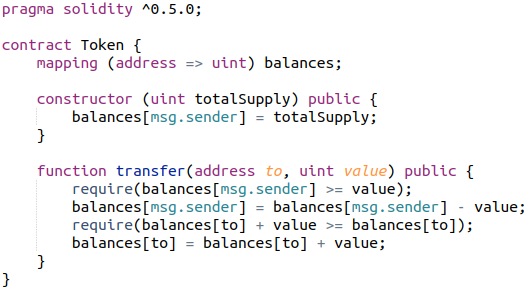
\includegraphics[scale=0.45,clip=false]{pictures/under-overflow-fixed-check.png}
    \end{center}
  \end{greenbox}
    
\end{frame}

\begin{frame}\frametitle{Over/underflows: prevention}

  \begin{greenbox}{Replace numerical operations with a library for safe arithmetic}
    \begin{center}
      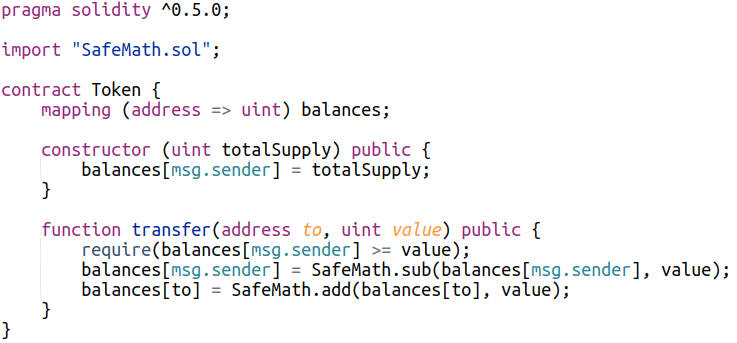
\includegraphics[scale=0.45,clip=false]{pictures/under-overflow-fixed.png}
    \end{center}
  \end{greenbox}
    
\end{frame}

\begin{frame}\frametitle{Over/underflows: prevention}

  \begin{greenbox}{A library for safe arithmetic}
    \begin{center}
      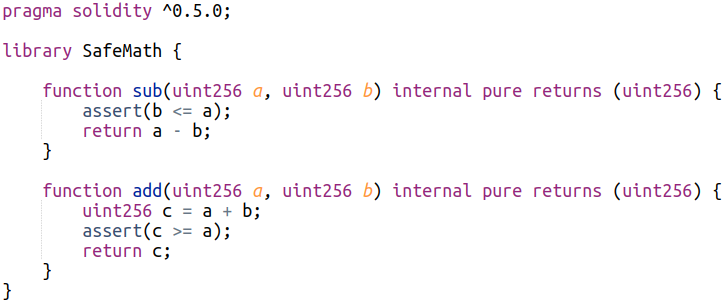
\includegraphics[scale=0.45,clip=false]{pictures/safe-math.png}
    \end{center}
  \end{greenbox}

  \medskip

  \begin{center}
    \url{https://docs.openzeppelin.com/contracts/2.x/api/math}
  \end{center}
  
\end{frame}

\begin{frame}\frametitle{Issue \#3: Unexpected ether}

  \begin{redbox}{}
    Code correctness depends on invariants about \<this.balance>,
    that actually do not hold.
  \end{redbox}

  \bigskip

  \begin{greenbox}{This code assumes \<this.balance \% 0.5 ether == 0>. But this is false
      since it is possible to send $0.1$ ether to this contract\ldots}
    \begin{center}
      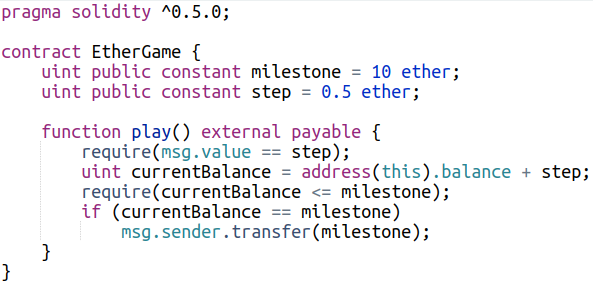
\includegraphics[scale=0.5,clip=false]{pictures/unexpected-ether.png}
    \end{center}
  \end{greenbox}

\end{frame}

\begin{frame}\frametitle{Issue \# 3: Unexpected ether}

  \begin{redbox}{}
    It is possible to send ether to a contract, without calling any \<payable> function
    nor its fallback function (if any)!
  \end{redbox}

  \bigskip

  \begin{greenbox}{How?}
    \begin{itemize}
    \item write a suicidal contract that executes \<selfdestruct(beneficiary)>
      and forwards its balance to \<beneficiary>: it does not even call
      the fallback function of \<beneficiary>!
    \item let ether be there from the very beginning, by sending ether
      to the address of the contract before its same creation!
      Remember that the address of a contract is computed deterministically
      from the address of the creator and from its current nonce
    \end{itemize}
  \end{greenbox}
  
\end{frame}

\begin{frame}\frametitle{Unexpected ether: prevention}

  \begin{greenbox}{Do not rely on \<this.balance>}
    Use your own counter instead.
  \end{greenbox}

  \bigskip

  \begin{center}
    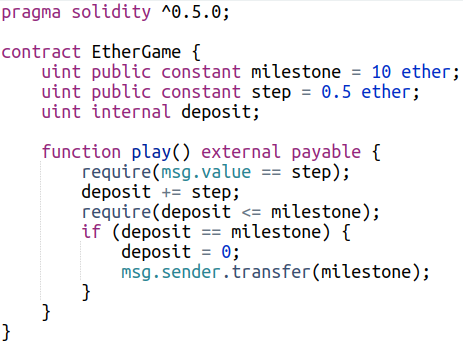
\includegraphics[scale=0.5,clip=false]{pictures/unexpected-ether-fixed.png}
  \end{center}  

\end{frame}

\begin{frame}\frametitle{Issue \#4: \<delegatecall>}

  It is a low-level call that allows one to call any method, as
  done in Java by reflection (and much worse).

  \bigskip

  \begin{redbox}{It keeps the calling context}
    If the callee reads/modifies its $n$th state variable, it actually
    reads/modifies the $n$th state variable of the caller, regardless of
    names and types.
  \end{redbox}

\end{frame}

\begin{frame}\frametitle{Example: storage slot clash}

  \begin{center}
    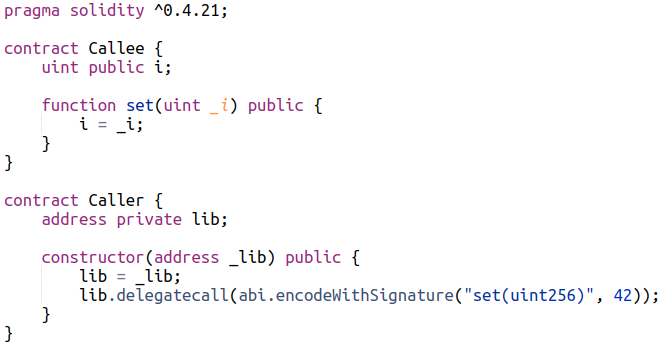
\includegraphics[scale=0.33,clip=false]{pictures/delegatecall-storage-clash.png}
  \end{center}

  Invoking the constructor of \<Caller> with the address of a \<Callee> \visible<2>{actually
  results in the \alert{\<private>} field \<lib> being set to $42$.

  \begin{center}
    
\includegraphics[scale=0.35,clip=false]{pictures/surprised-cat.jpg}
  \end{center}}

\end{frame}

\begin{frame}\frametitle{Example: call injection}

  \begin{center}
    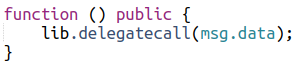
\includegraphics[scale=0.5,clip=false]{pictures/delegatecall-call-injection.png}
  \end{center}

  The caller can forge proper data so that \<delegatecall> ends up calling
  everything!

  \bigskip

  The same can occur with all low-level calls.

\end{frame}

\begin{frame}\frametitle{\<delegatecall>: prevention}

  \begin{greenbox}{}
    \begin{itemize}
    \item use it only on \<library>s: they cannot have state, hence they do not read/modify fields
      \begin{itemize}
      \item double-check that the receiver cannot be injected
      \end{itemize}
    \item use it with prepared call data only, to avoid call injections
    \item let the compiler, not you, use it, to compile calls to \<library>s
    \end{itemize}
  \end{greenbox}

\end{frame}

\begin{frame}\frametitle{Issue \#5: Weak encapsulation}

  \begin{greenbox}{}
    Programmers tend to be too permissive about visibility modifiers, often because
    they get along with the default \<public> visibility.
  \end{greenbox}

  \begin{center}
    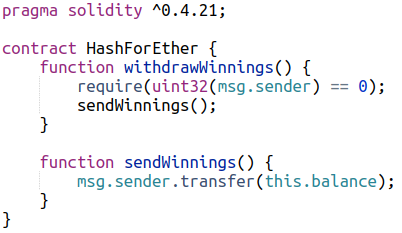
\includegraphics[scale=0.45,clip=false]{pictures/weak-visibility.png}
  \end{center}

  \begin{redbox}{}
    Everybody can call \<sendWinnings()>, it is \<public> by default!
  \end{redbox}

  \begin{greenbox}{}
    Too stupid? Don't overestimate the intelligence of
    programmers: somebody stole $\$31\text{M}$ from
    a slightly more complex contract.
  \end{greenbox}

\end{frame}

\begin{frame}\frametitle{Weak encapsulation: prevention}

  \begin{itemize}
  \item be the stricter as you can about visibility
    \begin{itemize}
    \item even \<internal> can be dangerous, because it is callable from
      subcontracts
    \end{itemize}
  \item beware of default visibility (\emph{ie.}, \<public>)
    \begin{itemize}
    \item latest compilers forbid default visibility
    \end{itemize}
  \item think seriously about the API of your contracts
  \end{itemize}
  
\end{frame}

\begin{frame}\frametitle{Issue \#6: Entropy illusion}

  \begin{redbox}{Nothing is really random in blockchain}
    Do not rely on \<block.number>, \<block.gaslimit>, \<block.timestamp> or \<now>
      as a source of randomness: they are (partially) controlled by the miner.
  \end{redbox}

  \begin{center}
    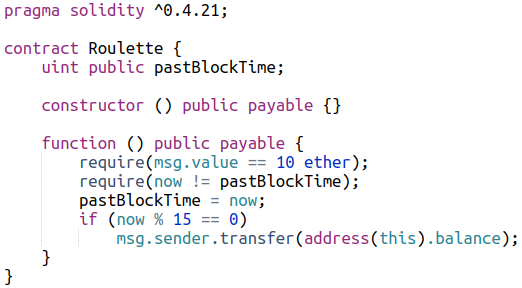
\includegraphics[scale=0.42,clip=false]{pictures/roulette.png}
  \end{center}

  The miner might choose \<now> so that the condition holds (or does not hold).
\end{frame}

\begin{frame}\frametitle{Entropy illusion: prevention}

  \begin{greenbox}{}
    \begin{itemize}
      \item use an external trusted \alert{oracle} as a source of randomness:
        \begin{description}
        \item[Oracle] A computer that regularly sends transactions that
          store data in blockchain. For instance, it sends and stores a random number.
        \end{description}
      \item if \<now> or \<block.timestamp> is used to wait for a period of time,
        it might be safer to wait for a specific blockchain height instead
    \end{itemize}
  \end{greenbox}
    
\end{frame}

\begin{frame}\frametitle{Issue \#7: External contract referencing}

  \begin{redbox}{}
    Casts and contract types are unchecked. Do not let clients
    inject contract types through the public API.
  \end{redbox}

  \medskip

  \begin{greenbox}{By injecting a malicious \<\_tail>, function \<length> might run
    arbitrary code}
  \begin{center}
    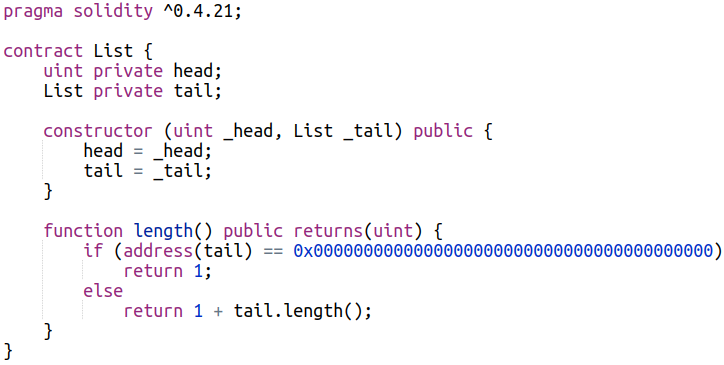
\includegraphics[scale=0.32,clip=false]{pictures/list.png}
  \end{center}
  \end{greenbox}

  \medskip

  \begin{redbox}{}
    This even compiles if \<length> is defined as \<view>, although it can have
    any possible side-effect.
  \end{redbox}

\end{frame}

\begin{frame}\frametitle{External contract referencing: prevention}

  \begin{itemize}
  \item avoid it!
  \item do not call functions on externally referenced contracts
  \item only talk to your friends!
    \begin{itemize}
    \item if \<field = new MyContract()> is the only way to initialize \<field>,
      then you can trust the type of \<field>
    \end{itemize}
  \end{itemize}
  
\end{frame}

\begin{frame}\frametitle{Issue \#8: Short address/parameter attack}

  \begin{redbox}{}
    Function parameters are encoded as transaction data. If shorter than
    expected, the encoding is silently padded with $0$'s.
  \end{redbox}

  \medskip

  \begin{greenbox}{How to buy a Porsche with $500$ euros}
    \begin{enumerate}
    \item generate private keys until the derived address \<A> ends in \<0x00>
    \item communicate the first $38$ digits \<A'> of \<A> to an exchange (without the
      two final \<0x00>), asking to buy $3$ ETH (as of today, $500$ euros)
    \item pay the exchange the $500$ euros (plus commission)
    \item its wallet will prepare a transaction to some
      \<transfer(address to, uint tokens)>, with data
      \<selector::A'::0x000000....00003::0x00>, where the final \<0x00> is padding
      to match the expected data size for \<transfer>
    \item the EVM will interpret the address as \<A'::0x00>, that is, \<A> (ours!)
    \item the EVM will interpret the \<tokens> parameter as $\<0x0000...000300>$, that is,
      $768$ ETH (as of today, $99,840$ euros)
    \item you will earn $99,840-500=99,340$ euros (minus commission)
    \end{enumerate}
  \end{greenbox}
  
\end{frame}

\begin{frame}\frametitle{Prevention: Short address/parameter attack}

  \begin{greenbox}{Spoiler: exchanges check consistency of data nowadays}
    \begin{center}
      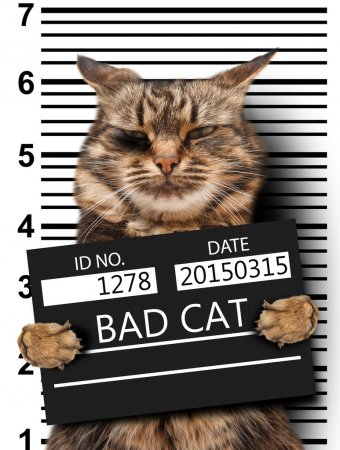
\includegraphics[scale=0.32,clip=false]{pictures/cat-jail.jpg}
    \end{center}
  \end{greenbox}

  \bigskip

  \begin{itemize}
  \item check parameters passed into blockchain
  \item use wallets to check basic consistency and warn otherwise
  \end{itemize}
  
\end{frame}

\begin{frame}\frametitle{Issue \#9: Unchecked return value}

  \begin{redbox}{}
    The return value of some functions (typically, \<send> and
    \<call>) should be checked, since it is a boolean
    that informs about their outcome.
  \end{redbox}

  \begin{center}
    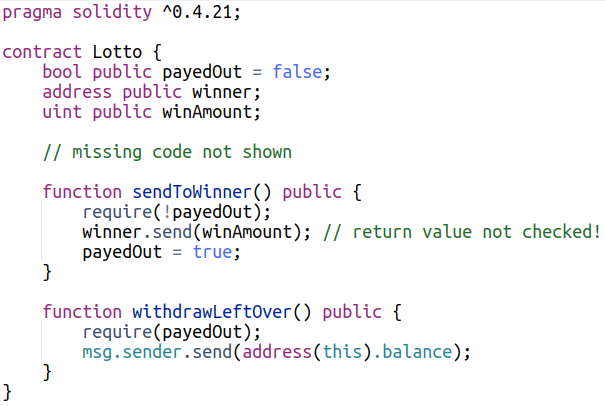
\includegraphics[scale=0.32,clip=false]{pictures/lotto.png}
  \end{center}

  \<payedOut> is set to true even if \<winner.send(winAmount)> fails.

  \begin{greenbox}{}
    Prevention: check the result of \<send> and \<call>. Use \<transfer> instead of \<send>.
  \end{greenbox}
\end{frame}

\begin{frame}\frametitle{Issue \#10: Race conditions/front running}

  \begin{redbox}{}
    Miners process transactions in the order they like (if ever);
    in general, they tend to proceed in decreasing \<gasPrice> order.
  \end{redbox}

  \bigskip

  \begin{greenbox}{Scenario \#1 (transaction ban, unlikely)}
    A miner could be instructed to never include a transaction that is
    detrimental to its owner. Unlikely to work for long, since it is practically impossible
    to be the fastest to mine the next block, always.
  \end{greenbox}

  \bigskip

  \begin{greenbox}{Scenario \#2 (transaction front running, likely)}
    A network sniffer could scan transactions, looking for
    those containing solutions to priced puzzles, and immediately
    place its own transaction with the same solution but a much higher \<gasPrice>,
    so that all miners will prefer to mine its transaction rather than the
    original one. The onwer of the sniffer will cash the price.
  \end{greenbox}

\end{frame}

\begin{frame}\frametitle{Front running example}

  \begin{center}
    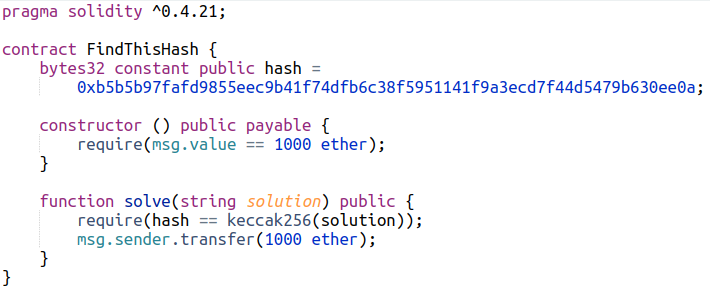
\includegraphics[scale=0.4,clip=false]{pictures/find-this-hash.png}
  \end{center}

  \begin{enumerate}
  \item clients try to guess the \<solution> whose hash is the given one
  \item a network sniffer scans all transactions, looking for calls to \<solve>
  \item for each call to \<solve>, the sniffer verifies if the solution is correct
  \item when, finally, a user submits the winning solution \<Ethereum!>, the sniffer
    realizes the user is going to win and immediately places its own transaction with the
    same solution but a very high \<gasPrice>
  \item miners will likely prefer its transaction to the original one
  \end{enumerate}
  
\end{frame}

\begin{frame}\frametitle{Prevention: race conditions/front running}

  \begin{itemize}
  \item at the level of protocol, the consensus rules might impose a maximal \<gasPrice>
  \item at the application level, solutions could be sent through
    the commit-reveal approach:
    \begin{enumerate}
    \item first a hashed solution is sent
    \item later, when no new solutions are allowed, the original image of the hash is revealed
    \end{enumerate}
    \begin{itemize}
    \item a big coding complication
    \item payable amounts should be hidden, or otherwise the sniffer might suspect
      something when seeing high amounts
    \item see the blind auction example
    \end{itemize}

  \end{itemize}
  
\end{frame}

\begin{frame}\frametitle{Issue \#11: Denial of service}

  \begin{redbox}{}
    If the cost of running transactions exceeds the block's gas limit, the
    transaction will never be executed, which might block a contract.
  \end{redbox}

  \begin{center}
    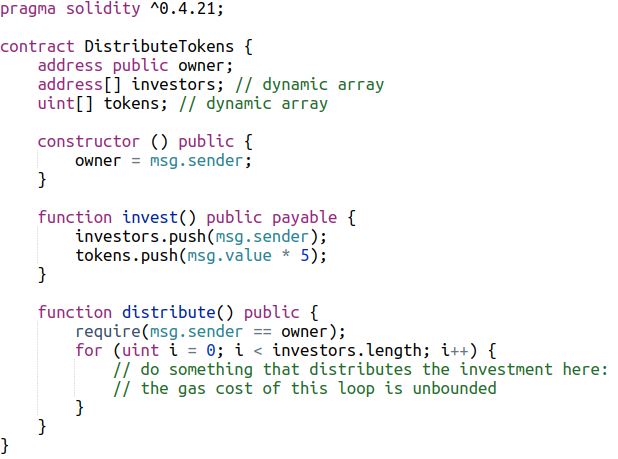
\includegraphics[scale=0.35,clip=false]{pictures/distribute-tokens.png}
  \end{center}

\end{frame}

\begin{frame}\frametitle{Prevention: denial of service}
  \begin{itemize}
  \item use the withdrawal pattern
  \item perform very cheap operations inside loops (no inner transactions, such as \<send>)
  \item impose an upper bound to the size of dynamic structures
  \end{itemize}
\end{frame}

\begin{frame}\frametitle{Issue \#12: Floating point imprecision}

  Solidity currently does not implement fixed nor floating-point arithmetic, hence
  integers are used instead.

  \medskip

  \begin{redbox}{}
    Beware of calculations that might lose precision! In particular: integer division.
  \end{redbox}

  \begin{center}
    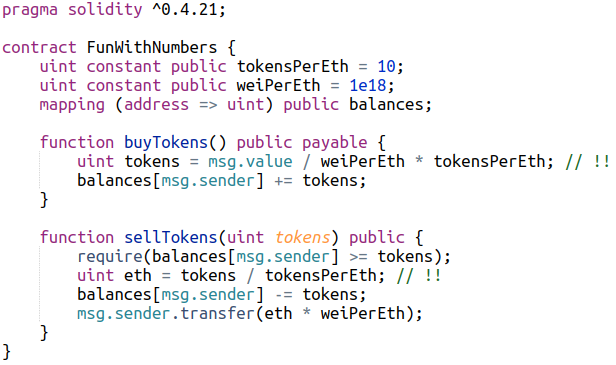
\includegraphics[scale=0.38,clip=false]{pictures/fun-with-numbers.png}
  \end{center}

\end{frame}

\begin{frame}\frametitle{Prevention: floating point imprecision}

  \begin{itemize}
  \item divide at the end:
    \<msg.value * tokensPerEth / weiPerEth>
    rather than \<\sout{msg.value / weiPerEth * tokensPerEth}>
  \item use libraries that simulate floating-point arithmetic
  \end{itemize}
  
\end{frame}

\begin{frame}\frametitle{Issue \#13: \<tx.origin> authentication}

  \begin{redbox}{}
    \<tx.origin> is the sender of the first transaction in a chain
    of transactions, not the sender of the current transaction (\emph{ie.}, it is not \<msg.sender>).
  \end{redbox}

  \begin{center}
    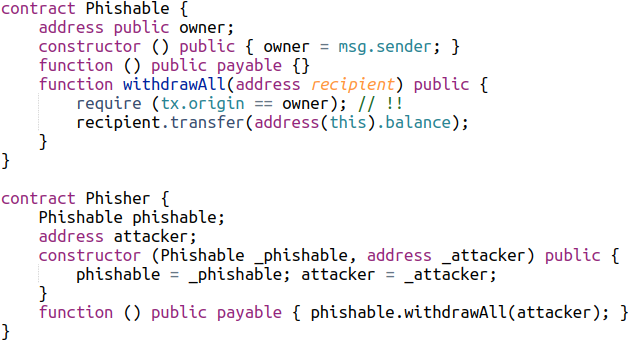
\includegraphics[scale=0.39,clip=false]{pictures/phishable.png}
  \end{center}

  \begin{enumerate}
  \item an \<attacker> identifies a \<phishable> in blockchain
  \item creates \<phisher = new Phisher(phishable, attacker)>
  \item convinces \<phishable.owner> to send ETH to \<phisher> and gets all! 
  \end{enumerate}

\end{frame}

\begin{frame}\frametitle{Prevention: \<tx.origin> authentication}

  \begin{itemize}
  \item it is almost always better to use \<msg.sender> instead of \<tx.origin>
  \item nevertheless, \<tx.origin> is legitimate sometimes:
    \<require(tx.origin == msg.sender)> prevents functions from being called
    from non-EOAs
  \end{itemize}
  
\end{frame}

\end{document}
